\section{ Data Warehouse}
\subsection{O que é um Data Warehouse}
Para \citeauthor{jmj} (\citeyear[p.12]{jmj}), um Data Warehouse é um repositório de informação coletada de múltiplas fontes, armazenados sobre um esquema definido e, geralmente, situado em um único local, assim, garantindo que a consistência dos dados, caso eles sejam acessados de locais diferentes. E esse local é mantido geralmente longe da base de dados operacional de uma organização \citep[p. 126]{jmj}. Eles suportam processamento de informações ao prover uma plataforma sólida de dados históricos para análise \citep[p. 126]{jmj}.

\subsection{Características de um Data Warehouse}
Segundo Inmon(1996), um DW é um conjunto de dados orientado por assuntos, integrado, variável com o tempo e não volátil, criados para dar suporte à decisão.

Orientado por assunto, ou seja, organizado em torno de um assunto principal. Ao invés de se concentrar nas operações diárias e no processamento de transações de uma empresa, um DW foca na modelagem e análise de dados para tomadores de decisões \citep[p. 126]{jmj}.

Integrado, um DW contém informações de fontes heterogêneas, como base de dados relacionais e flat files. Processos de data integration e data cleaning são aplicados para garantir consistência dos dados \citep[p. 126]{jmj}.

Variável com o tempo, armazena informações históricas dos últimos 5-10 anos, por exemplo.Toda estrutura chave em um DW contém, implicitamente ou explicitamente, um elemento de tempo \citep[p. 127]{jmj}.

E por último, não volátil, os dados não precisam ser alterados, já que um DW é fisicamente separado do ambiente operacional. As únicas operações realizadas em um DW são: carga inicial e acesso aos dados \citep[p. 127]{jmj}.

\subsection{Modelos de Data Warehouse}
Segundo \citeauthor{jmj} (\citeyear[p. 132]{jmj}) um DW pode ser dividido em três modelos, enterprise warehouse, data marte e virtual warehouse.

\subsubsection{Enterprise Warehouse}
Para \citeauthor{jmj} (\citeyear[p. 132]{jmj}), um enterprise warehouse coleta informações sobre um assunto que abrange toda uma organização . Ele fornece integração de dados em escala corporativa, geralmente de um ou mais sistemas operacionais ou de provedores de informação externos. Ele contém dados detalhados e sumarizados e podem variar de alguns poucos gigabytes para centenas de gigabytes.

Um enterprise warehouse é um conglomerado das data warehouse staging e presentation areas de uma organização (kimball2, p.8)



\subsubsection{Data Mart}
Segundo \citeauthor{jmj} (\citeyear[p. 132]{jmj}) um data mart contém um subconjunto de dados de uma escala corporativa e tem o escopo limitado a assuntos específicos.

Os dados podem ser independentes ou dependentes. Caso sejam independentes, os dados tem como fonte um ou mais sistemas operacionais ou provedores de informação externos. No caso de serem dependentes, os dados contidos no data mart são fornecidos diretamente de um enterprise warehouse.

\subsection{Componentes}

\subsubsection{Data Staging Area}
Para Krish Krishnan(p. 149), a staging area é outra base de dados que é construída e implementada em todo data warehouse com o propósito de juntar dados para qualidade dos dados e preparação dos dados, para, no fim, carregar os dados no DW. Já Kimball2 (p.8) diz que é tanto uma área de armazenamento como um conjunto de processos conhecidos como extract-transformation-loading (ETL). Esse processo será melhor explicado mais pra frente.

Existem diversas formas de carregar dados na staging area, como flat files, xml, modelos relacionais.

A staging area geralmente é composta de um database management system (DBMS) e arquivos de texto (flat files) \citep[p. 35]{jmj}. Em muitos casos, os dados precisam ser armazenados fora de um DBMS, em flat files, para um rápido processamento sequencial \citep[p. 35]{jmj}. Flat files contém dados armazenados em linhas e colunas \citep[p. 36]{jmj}.
\citeauthor{rk} (\citeyear[8]{rk} descreve o primeiro passo na criação (extração) de um data staging area como a leitura e entendimento da fonte de dados e copiar o que for necessário para manipulação futura.

Segundo \citeauthor{rk} (\citeyear[8]{rk}), quando os dados são extraídos , existem diversas transformações que podem ser realizadas, como limpeza e combinar dados de diferentes fontes. Essas transformações acontecem antes de carregar os dados na presentation area.

\subsubsection{Data Presentation Area}
A presentation area é onde os dados estão organizados, armazenados e disponíveis para consulta por usuários ou alguma aplicação analítica de Business Intelligente (BI) \citep[21]{rk}. Ele também afirma que a modelagem dimensional é a técnica mais viável para entregar dados aos usuários de DW/BI.

Ele deve conter dados atômicos detalhados \citep[21]{rk}  Embora a presentation area contenha dados agregados, é completamente inaceitável que somente dados sumarizados sejam armazenados enquanto os dados atômicos estão trancados em modelos normalizados. \citep[21]{rk}. Os dados mais finamente granulados devem ser apresentados na presentation area para que usuários possam fazer as perguntas mais precisas.

\subsection{Extract, Transform, Load (ETL)}
O processo de extract, transform, load (extrair, transformar, carregar) também conhecido como ETL é um processo utilizado para a construção de data warehouses. O sistema ETL é tudo entre os sistema de fontes operacionais e a presentation area de um DW \citep[19]{rk}. 

O primeiro passo é a extração dos dados, é esperado que o sistema tenha que extrair dados de uma grande variedade de fontes \citep[453]{rk}. As organizações podem extrair dados de fontes como arquivos xml, banco de dados, planilhas e etc.

O segundo passo é a transformação, após os dados serem extraídos, diversas transformações podem ser realizadas, como limpeza, combinar dados de fontes diversas e duplicação dos dados \citep[20]{rk}.

Essa limpeza pode, segundo \citeauthor{rk} (\citeyear[455]{rk}) mudar os dados e aperfeiçoar o seu valor para uma organização. Ou seja, corrigir problemas como um campo de telefone que está em diferentes formatos, quando retirados de fontes diferentes.

O terceiro, e último, passo é o carregamento, que é o processo de estruturar fisicamente e carregar os dados dentro dos modelos dimensionais da presentation area \citep[20]{rk}.

\section{CRISP-DM}
\subsection{O que é CRISP-DM}
CRISP-DM, ou Cross-industry standard process for data mining, é uma técnica utilizada no processo de mineração de dados, com uma série de tarefas a serem realizadas para chegar ao melhor resultado.

Segundo \citeauthor{dmfd} (\citeyear[75]{dmfd}), mineração de dados não é algo feito uma vez e depois esquecido, o trabalho pode ser aplicado em outros projetos, pode servir de referência

O ciclo de vida da mineração de dados contém seis fases, como apresentado na figura 1: entendimento do negócio, entendimento dos dados, preparação dos dados, modelagem, avaliação e implementação. 
A mineração de dados não termina uma vez que a solução é implementada \citep[10]{crispmanual}

\begin{figure}[h]
\centering
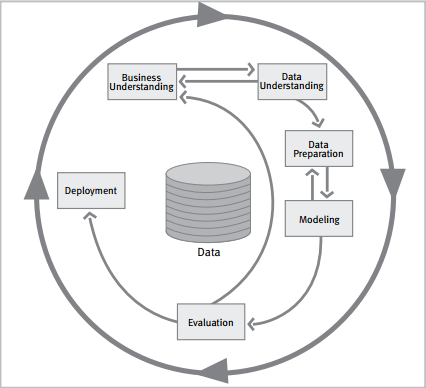
\includegraphics[height=6.2cm]{imagens/lifecycle.png}
\caption{teste}
\label{fig:exemplo}
\end{figure}

Cada uma dessas fases tem diversas tarefas que são realizadas para completar cada uma das fases e cada tarefa tem suas saídas.

\subsection{Entendimento do negócio}
A primeira fase do CRISP-DM é o entendimento do negócio, que foca em entender os objetivos do negócio e seus requerimentos de uma perspectiva de negócio.

As tarefas que compõe essa fase são: 
\begin{enumerate}
    \item determinar o objetivo do negócio;
    \item avaliar a situação;
    \item determinar os objetivos da mineração de dados;
    \item produzir um plano de projeto
\end{enumerate}

\subsubsection{Determinar o Objetivo do Negócio}
O primeiro objetivo da analise de dados é entender, sob uma perspectiva de negócio, o que o cliente deseja realizar. Segundo \citeauthor{dmfd} (\citeyear[76]{dmfd}), deve ter um entendimento claro do problema que deseja abordar, o objetivo do negócio, as limitações e o impacto.

Com isso, será possível produzir as saídas, que são \textbf{background}: informação da situação do negócio no início do projeto, \textbf{objetivos do negócio}: o objetivo primário do cliente e \textbf{critério de sucesso do negócio}: um critério para um resultado de sucesso do projeto \citep[14]{crispmanual}.

\subsubsection{Avaliar a Situação}
Essa tarefa consiste em um detalhamento maior dos recursos, limitações, premissas e outros fatores que devem ser considerados ao determinar os objetivos da análise de dados e do plano de projeto \citep[14]{crispmanual}.

As saídas dessa tarefa são um:
\begin{itemize}
    \item inventário de recursos: lista de todos os recursos pessoais, de dados e softwares disponíveis;
    \item requerimentos, premissas e limitações: listar todos os requerimentos do projeto, premissas e limitações do projeto;
    \item riscos e contingências: listar eventos que podem atrasar o projeto e os planos de contingência para esses riscos;
    \item terminologia: um glossário com os termos de negócio e de mineração de dados;
    \item custos e benefícios: uma análise de custo benefício do projeto. Segundo Meta S. B. (94), se os benefícios não exceder os custos de forma significante, pare e reconsidere essa análise e o projeto
\end{itemize}

\subsubsection{Determinar os Objetivos da Mineração de Dados}
Objetivos da mineração de dados em termos técnicos \citep[16]{crispmanual}. Determinar o que deseja alcançar por meio da mineração de dados, como "prever quantas pessoas irão visitar uma loja no verão, de acordo com informações dos últimos 2 anos dessa loja"

As saídas são:
\begin{itemize}
    \item Objetivos da mineração de dados: descrever as saídas desejada que permita alcançar o objetivo do negócio \citep[17]{crispmanual}.
    \item Critério de sucesso da mineração de dados: critério técnico de sucesso, como um certo nível de precisão.
\end{itemize}

\subsubsection{Produzir Plano de Projeto}
Descrever o plano desejado para atingir os objetivos da mineração de dados e desse modo, os objetivos do negócio \citep[17]{crispmanual}.
As saídas são: 
\begin{itemize}
    \item Plano de Projeto: Lista de estágios que serão executados no projeto, recursos necessários, entradas e saídas para cada passo e etc. O plano de projetos deve conter planos detalhados para cada fase \citep[17]{crispmanual}.
    \item Avaliações iniciais de ferramentas e técnicas: Deve ser feito no final da primeira fase
\end{itemize}

\subsection{Entendimento dos dados}
Segundo \citeauthor{dmfd} (\citeyear[79]{dmfd}), na segunda fase do projeto de mineração de dados, os dados tem que ser obtidos e tem que verificar se eles são apropriados para as necessidades.
As tarefas dessa fase são:
\begin{enumerate}
    \item Coletar dados iniciais;
    \item Descrever os dados;
    \item Explorar os dados;
    \item Verificar a qualidade dos dados.
\end{enumerate}

\subsubsection{Coletar Dados Iniciais}
Adquirir os dados listados nos recursos do projeto \citep[18]{crispmanual}. É necessário realizar o carregamento dos dados em alguma ferramenta, como o Pentaho, se for necessário para o entendimento dos dados.

A saída é: 
\begin{itemize}
    \item Relatório da coleta inicial de dados: Listar todos os datasets adquiridos, junto com suas localizações, métodos utilizados para aquisição e problemas encontrados. 
\end{itemize}
\subsubsection{Descrever os dados}
Examinar os dados adquiridos e relatar os resultados.
A saída é:
\begin{itemize}
    \item Relatório da descrição dos dados: Descrever os dados, como o formato em que eles se encontram, por exemplo.
\end{itemize}

\subsubsection{Explorar os dados}
Explorar os dados utilizando técnicas de visualização. Essa análise pode estar diretamente ligada aos objetivos da mineração de dados \citep[18]{crispmanual}.
A saída é:
\begin{itemize}
    \item Relatório da exploração de dados: descrever os resultados dessa tarefa, descobertas iniciais ou hipóteses, e o seu impacto no restante do projeto \citep[19]{crispmanual}. Esse relatório deve conter uma descrição mais detalhada dos dados, incluindo distribuições, sumários ou quaisquer sinais de problemas com a qualidade dos dados\citep[81]{dmfd} .
\end{itemize}
\subsubsection{Verificar a Qualidade dos Dados}
Examinar a qualidade dos dados para responder perguntas como "os dados estão completos?", "existem valores faltantes?" e etc.
A saída é: 
\begin{itemize}
    \item Relatório da qualidade dos dados: Listar o resultado da verificação, listar os problemas encontrados e suas soluções.
\end{itemize}
\subsection{Preparação dos Dados}
A maior parte do tempo gasto no processo de mineração de dados é na preparação deles, já que diversos tratamentos precisam ser feitos nos dados e isso nem sempre é tão simples. A maior parte dos dados usados para mineração foram originalmente coletados e preservados para outros objetivos e precisa ser refinado antes de ser ficar pronto para a modelagem \citep[82]{dmfd}.

As tarefas para essa fase são:
\begin{enumerate}
    \item Selecionar os dados
    \item Limpar os dados
    \item Construir dados
    \item Integrar dados
    \item Formatar dados
\end{enumerate}
Essa fase tem duas saídas, antes das tarefas, que são: \textbf{datasets}, que são os dados produzidos nessa fase e serão usados para modelagem e \textbf{descrição do dataset} \citep[21]{crispmanual}.
\subsubsection{Selecionar os dados}
Selecionar os dados que serão utilizados na modelagem, baseado nos objetivos da mineração de dados, qualidade e limites técnicos \citep[21]{crispmanual}.
Nessa fase é preciso também selecionar os atributos e linhas da tabela.
A saída é:
\begin{itemize}
    \item Razão para inclusão e exclusão: uma lista dos dados que foram incluídos/excluídos e a razão, que pode ser a qualidade, relevância para o projeto, limitações de linhas e colunas.
\end{itemize}
\subsubsection{Limpar os dados}
Elevar a qualidade dos dados para o nível requerido pelas técnicas de analise selecionadas \citep[21]{crispmanual}.
Segundo \citeauthor{dmfd} (\citeyear[83]{dmfd}), dificilmente os dados selecionados estarão perfeitamente limpos, mudanças precisarão ser feitas nos dados para atingir o nível necessário.
A saída é:
\begin{itemize}
    \item Relatório de limpeza de dados: Descrever as ações tomadas para lidar com os problemas encontrados anteriormente. \citeauthor{crispmanual} (\citeyear[21]{crispmanual}) diz que transformações nos dados podem ser feitas para limpeza e possível impacto na análise de resultados.
\end{itemize}
\subsubsection{Construir dados}
Essa tarefa consiste na criação de novos campos, dados agregados, ou novos formatos de dados. 
As saídas são:
\begin{itemize}
    \item Atributos derivados: Atributos criados a partir de dois ou mais atributos que já existem, necessário explicar como e por que foram criados.
    \item Registros gerados: Um relatório que explica por que e como novos registros foram criados. Eles podem não ser muito úteis antes, mas podem ser extremamente valiosos para a mineração de dados.
\end{itemize}
\subsubsection{Integrar Dados}
Os dados podem estar em diferentes datasets e é necessário a integração desses dados para a fase de modelagem.
A saída dessa fase é:
\begin{itemize}
    \item Dados fundidos: Fundir tabelas se refere a juntar duas ou mais tabelas que tem diferentes informações sobre o mesmo objeto \citep[22]{crispmanual}. Agregações também podem ser feitas para fundir os dados, ou seja, computar novos valores sumarizados de diversos registros.
\end{itemize}
\subsubsection{Formatar dados}
Dados frequentemente vem em formatos que não são os convencionais para modelagem \citep[83]{dmfd}, então conversões precisam ser feitas. Essas conversões não mudam o seu significado. \citeauthor{dmfd} (\citeyear[84]{dmfd}) afirma que a fase de preparação de dados deve ser finalizada com um dataset pronto para modelagem e um relatório descrevendo o dataset.
A saída é: 
\begin{itemize}
    \item Dados reformatados: Os dados reformatados, convertidos para alguma unidade de medida única para todos os dados (como quilos, em peso).
\end{itemize}
\subsection{Modelagem}
É a fase onde alguma técnica de aprendizado de máquina é utilizada, testada e avaliada para encontrar padrões nos dados, como K-nearest neighbors, Decision Tree e etc.

As tarefas dessa fase são:
\begin{enumerate}
    \item Selecionar técnica de modelagem
    \item Gerar teste de design
    \item Construir o modelo
    \item Avaliar o modelo
\end{enumerate}
\subsubsection{Selecionar técnica de modelagem}
O primeiro passo da modelagem é selecionar a técnica de modelagem que será usada, caso múltiplas técnicas sejam aplicadas, é necessário executar essa tarefa para cada uma delas \citep[24]{crispmanual}.
Nem todas as técnicas de modelagem serão uteis para as necessidades do negócio.
As saídas dessa fase são:
\begin{itemize}
    \item Técnica de modelagem: a técnica que será utilizada
    \item Hipóteses da modelagem: As técnicas de modelagem fazem vários hipóteses sobre os dados, é necessário registrar elas \citep[24]{crispmanual}.
\end{itemize}
\subsubsection{Gerar teste de design}
Antes de construir o modelo, é necessário gerar procedimentos ou mecanismos para testar a qualidade e validade do modelo \citep[24]{crispmanual}. Os dados geralmente são separados em dois conjuntos, o conjunto de treinamento e o conjunto de teste. 
O conjunto de treinamento é usado para construir o modelo e o de teste para validar ele.
A saída é:
\begin{itemize}
    \item Design de teste: descreve como planeja treinar, testar e avaliar o modelo.
\end{itemize}
\subsubsection{Construir o Modelo}
Rodar a ferramenta de modelagem para criar um ou mais modelos \citep[24]{crispmanual}.
As saídas são:
\begin{itemize}
    \item Configurações de parâmetros: Documentar as configurações dos parâmetros usados, já que as ferramentas oferecem uma grande quantidade de parâmetros.
    \item Modelos: os modelos produzidos pela ferramenta de modelagem.
    \item Descrição dos modelos: descrever os modelos, o tipo, as variáveis usadas, como ele é interpretado. 
\end{itemize}
\subsubsection{Avaliar o modelo}
Rever o modelo de um ponto de vista técnico e de negócio:
As saídas são:
\begin{itemize}
    \item Avaliação dos modelos: Sumarizar os dados, ranquear os modelos utilizados.
    \item Revisar as configurações dos parâmetros: revisar os parâmetros utilizados e tentar ajusta-los até encontrar a configuração que talvez seja a melhor possível.
\end{itemize}
\subsection{Avaliação}
Avaliar todo o processo, não só os modelos mas também o processo utilizado para a sua criação.
As tarefas para essa fase são:
\begin{enumerate}
    \item Avaliar Resultados
    \item Rever Processo
    \item Determinar próximos passos
\end{enumerate}
\subsubsection{Avaliar Resultados}
Essa tarefa avalia o grau em que o modelo se adequa a o objetivo original do negócio e busca determinar se existe alguma razão para o modelo estar deficiente.
As saídas são: 
\begin{itemize}
    \item Avaliação do resultado da mineração de dados a respeito do critério de sucesso do negócio: Sumarizar os resultados de acordo com o critério de sucesso. \citeauthor{dmfd} (\citeyear[86]{dmfd}) afirma que essa tarefa serve para dizer se o projeto atingiu ou não os objetivos definidos no início.
    \item Modelos Aprovados: Selecionar os modelos que atingiram o critério selecionado.
\end{itemize}
\subsubsection{Rever Processo}
Nesse ponto, os modelos resultantes aparentam ser satisfatórios para a necessidade do negócio \citep[27]{crispmanual}. Essa é uma fase usada para rever o processo, como algum problema que foi negligenciado. 
A saída dessa fase é:
\begin{itemize}
    \item Revisão do processo: \citeauthor{crispmanual} (\citeyear[27]{crispmanual}) diz que se deve sumarizar a revisão e ressaltar as atividades que não foram realizadas e aquelas que devem ser repetidas.
\end{itemize}
\subsubsection{Determinar próximos passos}
A fase de avaliação é concluída com as recomendações para o próximo passo \citep[87]{dmfd}. Decidir se deve finalizar o projeto ou continuar o desenvolvimento. Essa fase também inclui a análise das despesas  e recursos restantes, que podem influenciar na decisão \citep[27]{crispmanual}.
As saídas dessa fase são:
\begin{itemize}
    \item Lista de possíveis ações: Listar as potências ações a serem feitas e as razões para cada uma delas. 
    \item Decisão: Descrever a decisão em como prosseguir, junto com a razão \citep[27]{crispmanual}.
\end{itemize}
\subsection{Implementação}
O objetivo dessa fase final é a implementação do modelo.
As tarefas dessa fase são: 
\begin{enumerate}
    \item Plano de Implementação
    \item Plano de monitoramento e manutenção
    \item Produzir relatório final
    \item Revisão do projeto
\end{enumerate}
\subsubsection{Plano de implementação}
Essa fase usa os resultados da avaliação e determina a estratégia de implementação \citep[28]{crispmanual}. 
A saída é:
\begin{itemize}
    \item Plano de Implementação: Sumarizar as estratégias para implementação, os passos necessários e como realizar.
\end{itemize}
\subsubsection{Plano de monitoramento e manutenção}
Segundo \citeauthor{dmfd} (\citeyear[88]{dmfd}), mineração de dados é um ciclo, então é necessário continuar envolvido com os modelos enquanto eles são integrados ao dia-a-dia. A preparação cuidadosa das estratégias de manutenção ajuda a evitar longos períodos desnecessários de uso incorreto dos resultados da mineração \citep[29]{crispmanual}.
A saída é:
\begin{itemize}
    \item Plano de Monitoramento e Manutenção: Sumarizar todas as estratégias de manutenção e monitoramento, incluindo os passos necessários para realiza-los \citep[29]{crispmanual}.
\end{itemize}
\subsubsection{Produzir Relatório Final}
No final do projeto, é necessário escrever um relatório que pode ser somente um sumário do projeto e das experiências ou uma apresentação final e compreensível dos resultados da mineração \citep[29]{crispmanual}.
As saídas são:
\begin{itemize}
    \item Relatório Final: Sumariza todo o projeto ao juntar todos os relatórios criados até o momento \citep[88]{dmfd}
    \item Apresentação Final: Encontro realizado na conclusão do projeto com seu cliente.
\end{itemize}
\subsubsection{Revisão do Projeto}
O time se reúne e discute o que deu certo e o que não deu, o que pode ser feito novamente e o que não pode e o que deve ser evitado \citep[88]{dmfd}.
A saída é:
\begin{itemize}
    \item Documentação de Experiência: Sumarizar a experiência ganha com o projeto, como erros e acertos, dicas de como selecionar os melhores modelos para situações semelhantes e etc.
\end{itemize}